% This is samplepaper.tex, a sample chapter demonstrating the
% LLNCS macro package for Springer Computer Science proceedings;
% Version 2.20 of 2017/10/04
%
\documentclass[runningheads]{llncs}
%
\usepackage{graphicx}
\usepackage{amsfonts}
\usepackage{makecell}
\usepackage[marginal]{footmisc}

\usepackage{pifont}
\usepackage{float}
\usepackage{amsmath}
\usepackage{amssymb}
\usepackage{bbding} 
\usepackage{fontawesome}

\usepackage{hyperref}
\hypersetup{hidelinks,
	colorlinks=true,
	allcolors=black,
	pdfstartview=Fit,
	breaklinks=true}



\renewcommand{\thefootnote}{}
% Used for displaying a sample figure. If possible, figure files should
% be included in EPS format.
%
% If you use the hyperref package, please uncomment the following line
% to display URLs in blue roman font according to Springer's eBook style:
% \renewcommand\UrlFont{\color{blue}\rmfamily}

\begin{document}
%
\title{CA-UNet: UNet-like Heterogeneous Architecture of CNN and Attention for Medical Image Segmentation
% \thanks{Supported by organization x.}
}
%
%\titlerunning{Abbreviated paper title}
% If the paper title is too long for the running head, you can set
% an abbreviated paper title here
%
\author{Jian Wang\inst{1} \and
Fei Qi\inst{1*} \and
Jianfei Wu\inst{2}  \and
Siqi Yan\inst{3}
% \and
% Knoll Alois\inst{1}
}

%
\authorrunning{Jian Wang et al.}
% First names are abbreviated in the running head.
% If there are more than two authors, 'et al.' is used.
%

% First names are abbreviated in the running head.
% If there are more than two authors, 'et al.' is used.
%

\institute{Xidian University, Xi'an, China 
% Xidian University, Xi'an , China \and
% Xidian University, Xi'an , China 
% \email{lncs@springer.com}\\
% \url{http://www.springer.com/gp/computer-science/lncs} \and
% ABC Institute, Rupert-Karls-University Heidelberg, Heidelberg, Germany\\
% \email{\{abc,lncs\}@uni-heidelberg.de}
}

%
\maketitle              % typeset the header of the contribution
%


\begin{abstract}
Medical image segmentation has wide applications and research value in the field of medical research and practice, greatly improving the efficiency and accuracy of disease diagnosis.In various types of medical segmentation tasks, the encoder-decoder U-shaped heterogenous architecture network, which integrates convolutional neural networks (CNN) and attention mechanisms, has achieved milestone achievements. It empowers the network with strong local feature extraction ability and long-term dependency modeling capability, and has achieved excellent performance in medical image segmentation.However, most of the current heterogeneous networks adopt independent convolutional layers or attention layers in various feature extraction modules, unable to effectively establish dependencies between local and global information, thus failing to fully exploit their advantages.Moreover, due to the small sample characteristic of medical images which often limits the learning capacity of the network model, this article applies full-scale skip connection based on the convolutional attention mechanism to the feature fusion of the encoder and decoder, thereby effectively enhancing the segmentation performance of the network. In experiments involving Synapse multi-organ segmentation(Synapse) dataset, the average DSC of the proposed network reached 84.43\%, and HD95 reached 15.69. At the same time, it showed excellent generalization ability in Automated cardiac diagnosis challenge(ACDC) dataset.
Code is available at \href{https://github.com/waungjian/CA-UNet.git}{https://github.com/waungjian/CA-UNet.git}



% \keywords{Medical image segmentation  \and Pure transformer \and Deep learning.}
\end{abstract}
%
%
%
\footnote{*Corresponding author}
% \footnote{$\dagger$ Work done as an intern in Huawei Technologies}

\section{Introduction}

Due to the great success of deep learning, CNNs, especially Fully Convolutional Networks (FCN)~\cite{long2015fully}, have been widely used in the field of medical image segmentation. Based on the FCN, U-Net~\cite{ronneberger2015u}, as the pioneer of medical image segmentation, has attracted the attention of many researchers with its symmetrical encoder-decoder framework. In this topology structure, the encoder is used to extract feature information of different scales from images, while the decoder fuses the feature information extracted by the encoder via cross-layer connections and restores it to the original input image size, making pixel-level semantic predictions. This network structure has achieved effective fusion of fine-grained information and semantic information in small-sample data, and achieved great success in various medical image segmentation tasks. In order to alleviate the loss of spatial information caused by downsampling, U-Net++~\cite{zhou2019unet++} and U-Net3+~\cite{huang2020unet} networks based on multi-scale information fusion mechanism and deep supervision have been proposed successively. These methods learn hierarchical representations from feature maps aggregated at multiple scales, thus obtaining more accurate segmentation results.In addition, the DeepLab~\cite{liang2015semantic,chen2017deeplab,chen2017rethinking,chen2018encoder} series of networks combined with Atrous convolution designed a multi-scale objective robust algorithm based on Atrous Spatial Pyramid Pooling (ASPP).
% many fields such as

Although CNN have powerful feature extraction capabilities, due to the inherent locality of their convolution operations, CNN-based medical image semantic segmentation networks still show certain limitations in modelling visual receptive fields and long-range dependencies. The emergence of the visual attention mechanism provides a novel and effective path to enhance the long-range modeling capacity of CNNs. Attention U-Net~\cite{oktay2018attention} first introduced the gated attention mechanism into the U-Net network, allowing the network to learn the complex relations between features across different scales and hierarchical levels. In the same year, Woo et al.~\cite{woo2018cbam} effectively combined channel attention (CA) and spatial attention (SA) to propose a novel and lightweight convolution block attention module (CBAM). This module can be flexibly embedded into deep CNNs for various application scenarios and tasks without introducing extra computational or parameter load. A large number of experiments have demonstrated the effectiveness and generalization capabilities of CBAM in tasks such as image classification and image segmentation.

The self-attention mechanism based on Transformer~\cite{vaswani2017attention} has achieved great success in the field of natural language processing(NLP) due to its exceptional ability to model long-range dependencies, paving a new research path in the field of computer vision. In~\cite{dosovitskiy2020image}, Visual Transformer (ViT) was proposed and applied for image classification tasks. It performs equivalently to CNN-based classification networks when pre-trained on large-scale datasets, showcasing the powerful ability of Transformers in global context modeling. To enhance ViT's local perception capabilities and handle super-resolution images, researchers designed the Swin Transformer~\cite{liu2021swin}, which has been successfully applied in fields like image object detection and semantic segmentation. A series of studies have adopted Transformers in the field of medical image segmentation, seeking to replace CNNs~\cite{cao2022swin,huang2022missformer}. However, due to the lack of key inductive biases inherent to CNNs, such as translation invariance and locality, its ability to extract spatial detail features is limited. Based on the complementary strengths of CNNs and ViTs, a series of hybrid U-shaped topologies based on CNN-ViT have been proposed for medical image segmentation tasks~\cite{chen2021transunet,zhang2021transfuse,naderi2022focal,lan2024brau}. A potential shortfall of these networks, however, is the lack of integration of the complementary strengths of both at each level of feature extraction modules, rendering them unable to effectively establish dependencies between local and global information. The exceptional performance of CMTs~\cite{guo2022cmt} in various visual tasks presents us with a novel method of hierarchical fusion between CNN-ViT.

Motivated by the success of the CMT architecture and the Swin Transformer~\cite{guo2022cmt,liu2021swin}, we propose CA-UNet for 2D medical image segmentation, including encoders, bottleneck, decoders, and full-scale skip connections. We combined the window attention mechanism unit in Swin Transformer with depthwise convolution (DwConv) based on a dynamic weight allocation mechanism to construct a parallel heterogeneous module (CA block). The encoders, bottleneck, and decoders are all built based on the CA block. First, spatial and structural information extraction is carried out on the input image stem architecture~\cite{he2019bag} and then input to the encoder for deep representation learning. The encoder obtains multi-scale feature maps based on a downsampling structure with residual architecture. Through the decoder and a full-scale skip connection module based on convolutional attention, the deep feature map extracted is fused with multi-scale features of different resolutions on the encoder path to achieve precise positioning. Numerous experiments on multi-organ and heart segmentation datasets have demonstrated the superiority of this method. Specifically, our contributions can be summarized as: (1) providing a novel U-shaped symmetric encoder-decoder architecture based on CNN and Transformer for medical image segmentation tasks based on parallel heterogeneous CA blocks; (2) a downsampling module based on residual architecture(Res block), which enhances key detail features of the downsampled feature map, further highlighting the hierarchical relationship of features; (3) a full-scale skip connection module based on CBAM, which allows the network to autonomously learn the importance of the encoder's feature information for decoders at different levels.

\section{Related work}

\subsubsection{CNN-based methods}:
Due to the powerful characterization capability of deep CNNs, researchers applied them to medical image segmentation tasks and proposed U-Net~\cite{ronneberger2015u}. Due to the superior performance and generalization ability of U-shaped structure, various networks based on U-shaped structure have also been proposed successively, such as U-Net++~\cite{zhou2019unet++} and U-Net3+~\cite{huang2020unet}, which incorporate multiscale mechanism, and Residual U-Net~\cite{baldeon2020adaresu,alom2018nuclei,mostafiz2018retinal,li2019automatic}, which incorporates residual connectivity. Some researchers have also applied the structure to the field of 3D medical image segmentation, and 3D U-Net~\cite{cciccek20163d} and V-Net~\cite{milletari2016v} have been proposed successively.

\subsubsection{Attention mechanism}:
The visual attention mechanism holds crucial significance in deep learning technology research. Attention U-Net~\cite{oktay2018attention} was the first to introduce the gated visual attention mechanism, enhancing the modeling capability of complex relationships between features at different scales and levels. U-Net v2~\cite{peng2023u} combines the CBAM module with the cross-layer connections of U-Net architecture, endowing the decoder's multi-level feature maps with rich semantic information and complex detail features through attention focus.With the great success of Transformer on natural language processing, many researchers applied it to computer vision tasks and proposed ViT~\cite{dosovitskiy2020image}. It was applied to image recognition tasks and achieved comparable performance to CNN with large-scale data pre-training. To improve the applicability of Transformer for various vision tasks, Swin Transformer~\cite{liu2021swin} with a hierarchical structure was created to bring higher efficiency through a multi-scale modeling and shifted windowing scheme, demonstrating the potential of Transformer-based models as a visual backbone. Based on the excellent performance of Transformer on vision tasks, combined with the U-shaped architecture, researchers proposed Swin-UNet~\cite{cao2022swin} for medical semantic segmentation tasks and achieved excellent segmentation accuracy, providing a new perspective to solve the problem of medical semantic segmentation tasks. To further enhance the adaptive feature alignment ability of the Transformer, researchers optimized its structure, applied it to U-Net's network encoder, decoder, and skip connections for feature extraction, and proposed MISSFormer~\cite{huang2022missformer} for use in medical image segmentation tasks.

\subsubsection{Combining CNNs with Transformer}:
Due to the excellent performance of Transformer in the field of vision, researchers have endeavored to combine CNN with Transformer and exploit the complementary nature of both to build U-shaped encoder-decoder medical image segmentation models and improve the segmentation capability of the models, such as TransUNet~\cite{chen2021transunet} and TransFuse~\cite{zhang2021transfuse}. Different from the fusion approach of the above hybrid architecture models, we try to explore the potential of a novel structural fusion approach of hybrid architecture in medical image segmentation. In addition, leveraging the outstanding global modelling ability of Transformer, CASTformer~\cite{you2022class} has built a class-aware module based on the Transformer, which updates the sampling positions through iterative optimization, thereby adapting to the key areas of objects, such as anatomical features and structural information.




\section{Method}

\subsection{Architecture overview}

The overall architecture of the proposed CA-UNet is presented in Fig.~\ref{ca_unet}.Its basic constituent units mainly include the following three parts: (1) The CA block that fuses convolution and attention mechanisms, used for constructing network feature extraction modules; (2) the downsampling module based on residual structure; (3) The full-scale skip connection module based on the convolution block attention mechanism. Given an input image $\pmb{X} \in \mathbb{R}^{H \times W \times C}$ with a spatial resolution of $H \times W$ and a channel number of $C$, it is first passed through a stem architecture~\cite{he2019bag} for image resolution reduction and fine-grained feature extraction. After downsampling, the image resolution drops to $\frac{H}{4} \times \frac{W}{4}$, and then it is input to a series of CA blocks for feature extraction and fusion. Downsampling in four stages generates feature maps of different scales, and these multi-scale feature maps are critical for feature extraction in the dense prediction task during the decoding stage. In order to reduce the loss of spatial information in the feature map during downsampling, after bilinear upsampling in the decoder part, spatial detail information and abstract semantic information are fused through the full-scale skip connection module. After four stages of upsampling and feature extraction and fusion, a pixel-level segmentation result map  $\hat{\pmb{Y}}\in \mathbb{R}^{H \times W \times K}$ with the same spatial resolution as the original image is output, where $K$ represents the number of segmentation categories.

\begin{figure}[htbp]
\includegraphics[width=\textwidth]{images/CAUNet.png}
\caption{The architecture of CA-UNet, which is composed of encoder, bottleneck, decoder and skip connections. Encoder, bottleneck and decoder are all constructed based on CA block.} \label{ca_unet}
\end{figure}



\subsection{Stem architecture}

At present, most ViTs linearly map the input image into a one-dimensional sequence after dividing it into non-overlapping image patches, but this method destroys the two-dimensional structure and spatial information within each patch. To overcome the limitations of linear mapping modeling, CA-UNet adopts a stem architecture, expecting to map the input image into different dimensions of nonlinear space to preserve as much spatial and structural feature information as possible.It mainly consists of convolution layers, Gaussian Error Linear Unit activation functions, and BN layers. Firstly, a 3 × 3 convolution layer with a stride of 2 is used to downsample the input image, generating a feature map with half the resolution and a channel dimension of 32. Subsequently, local feature extraction is performed using two consecutive 3 × 3 convolution layers with a stride of 1.

\subsection{Parallel heterogeneous module}

Convolutional neural networks use self-learning convolution kernels to aggregate spatial information representation. The convolution operation, due to its translation invariance, can more effectively explore the potential representational capacity in feature channel dimensions, demonstrating superior local perception ability when analyzinge image spatial structure information. The key advantage of Transformer~\cite{vaswani2017attention} lies in its self-attention mechanism, which gives it exceptional capabilities in modeling long-range dependencies. In~\cite{vaswani2017attention,liu2021swin}, the self-attention mechanism associates features of different positions through a dynamic weight allocation mechanism. Without disrupting the respective structures and modeling of both, CA-UNet proposes a parallel heterogeneous module based on convolution and self-attention mechanisms, named CA block. It combines the advantages of both, adaptively allocating dynamic weights to different spatial positions and channel dimensions, thereby effectively capturing complex patterns in medical image feature maps.The CA Block primarily consists of parallel units composed of multi-head self-attention units based on the Swin Transformer~\cite{liu2021swin} and local perception units based on deep convolution, as well as the Inverted Residual Feed-forward Network (IRFFN)~\cite{guo2022cmt}. The module is shown in Fig.~\ref{ca_block}, and each of its components will be briefly introduced below.


\begin{figure}[htbp]
    \centering
    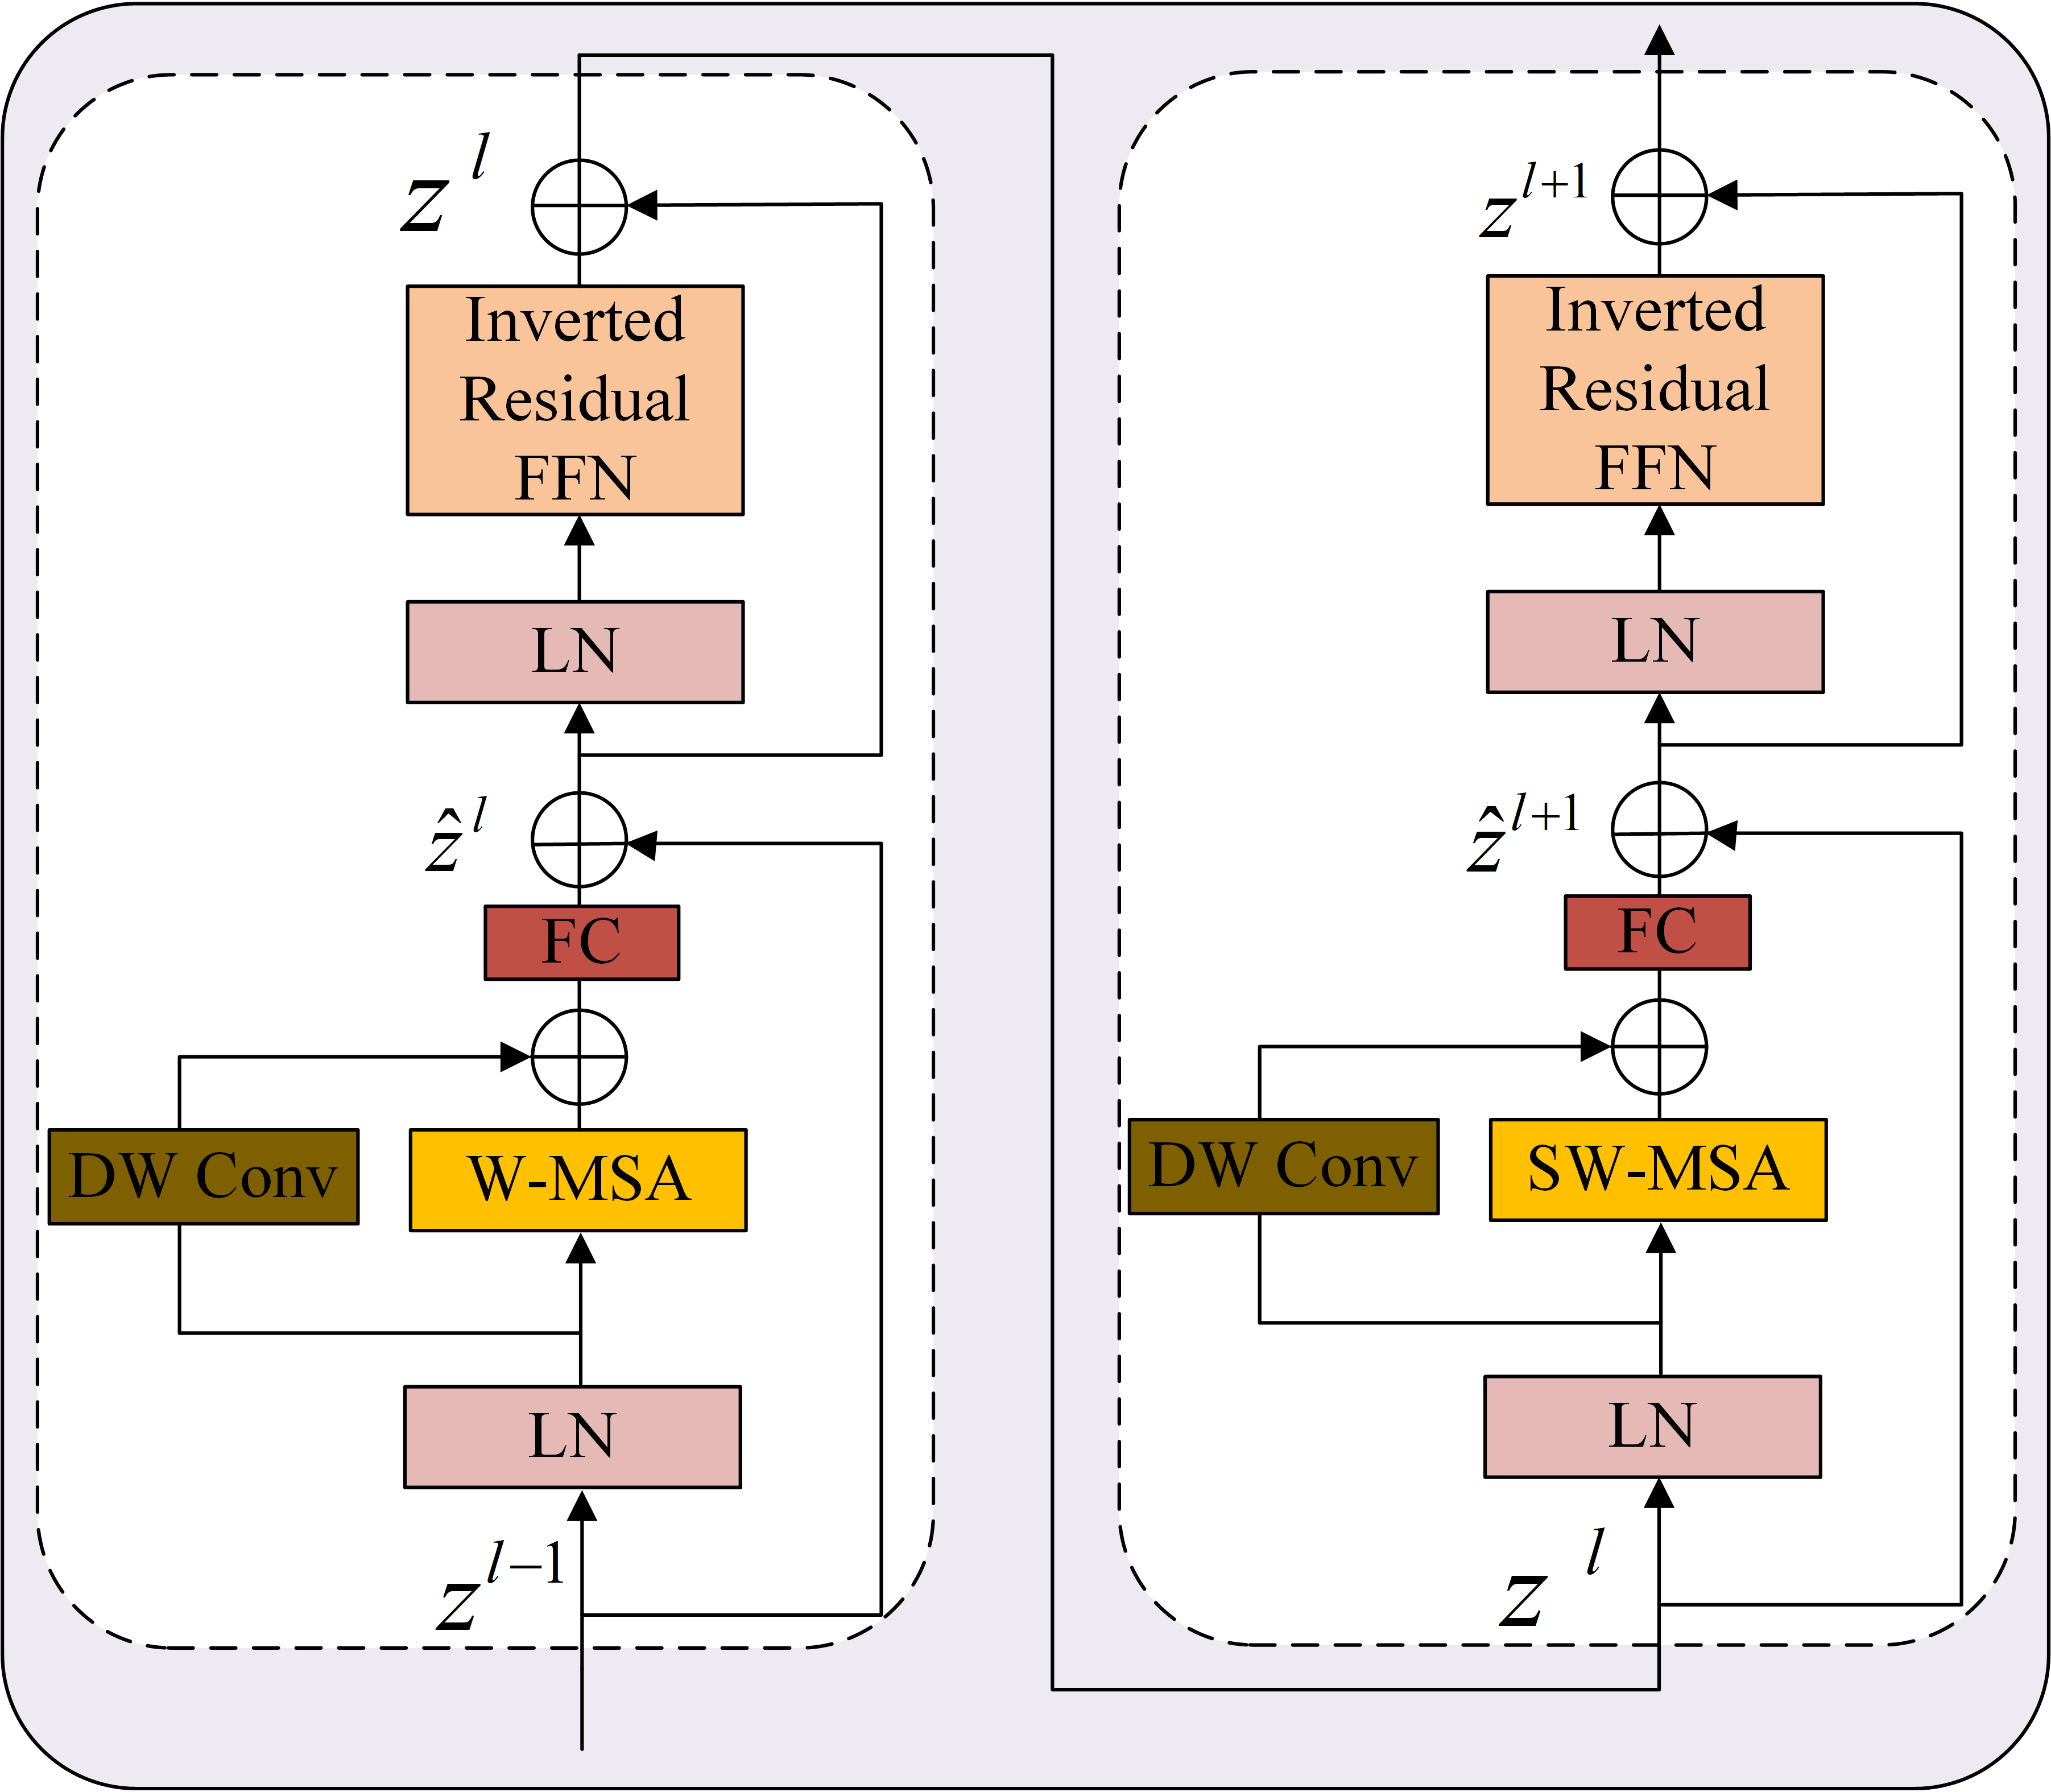
\includegraphics[width=0.8\textwidth]{images/ca_block.png}
    \caption{CA block.} \label{ca_block}
    \end{figure}

\textbf{Self-attention unit}\quad CA-UNet utilizes the window attention mechanism of the Swin Transformer~\cite{liu2021swin} with a multi-layer hierarchical architecture, effectively analyzing and extracting local features and global semantic information from medical images, while also reducing computational complexity. The W-MSA module divides the input image into non-overlapping windows for local self-attention calculation, and the window size is defaultly set as $7 \times 7$. This strategy helps reduce computational complexity and allows the model to handle larger scale images. The SW-MSA module re-divides the non-overlapping windows from the W-MSA stage using moving windows, effectively solving the receptive field limitation problem brought by the window attention mechanism. This strategy enables windows to have cross-window information interaction capability and expands their coverage range, thereby facilitating the model to better capture global information.  Similar to the previous works~\cite{raffel2020exploring,bao2020unilmv2,hu2018relation,hu2019local}, self-attention is computed as follows:

\begin{equation}
	\label{eq:swin_attention}
	\operatorname{Attention}(Q, K, V)=\operatorname{Softmax}\left(\frac{Q K^{T}}{\sqrt{d}}+B\right) V,
\end{equation}where $Q,K,V \in \mathbb{R}^{M^2 \times d}$ denote the query, key, and value matrices. $M^2$ and $d$ represents the number of patches in a window and dimension of the query or key,respectively. And the value in B are taken from the bias matrix   $\hat{\pmb{B}} \in \mathbb{R}^{(2 M-1) \times(2 M-1)}$

\textbf{Local perception unit}\quad This unit uses DwConv to enhance the local information perception of defect features in composite components, effectively exploring its potential representation capability in the feature channel dimension, while significantly reducing the amount of parameters and computational complexity. Considering the scale consistency of the window attention mechanism, the convolution kernel size is set to $7 \times 7$.

\textbf{Inverted Residual Feedforward Network}\quad The design of the IRFFN is similar to the inverse residual block~\cite{sandler2018mobilenetv2}, mainly composed of expansion layers, DwConv, and projection layers. The network enhances the ability of gradient propagation across layers while optimizing network performance by changing the position of skip connections. Notably, the IRFFN omits the activation layer and achieves efficient local feature extraction through DwConv, and the related additional computational cost is negligible. This structure is computed as follows:

\begin{equation}
	\begin{aligned}
		\label{eq:irffn}
		IRFFN\left( X \right) &= Conv\left( F \left( Conv \left(  X \right)  \right) \right), \\
		F\left( X \right) &= DwConv\left( X \right) + X.
	\end{aligned}
\end{equation}

Overall, the CA Block reconsiders the fusion strategy of CNN and Transformer based on the dynamic weight allocation mechanism, and achieves the complementarity and information synchronization of the two through fully connected layers (FC). Finally, it uses IRFFN to further capture the local structural features and global semantic information of the intermediate features, thereby enhancing the network's expressive ability. The CA Block is computed as follows:


\begin{equation}
	\begin{aligned}
		\label{eq:error-mae}
		\hat{z}^{l} &= \mathrm{W \text{-} M S A}\left(\mathrm{L N}\left(z^{l-1}\right)\right) + \mathrm{DwConv} \left(  \mathrm{LN} \left(  z^{l-1} \right) \right), \\
		z^{l} &= \mathrm{I R F F N}\left(\mathrm{L N}\left( \mathrm{FC} \left( \hat{z}^{l}  \right) \right) +  \hat{z}^{l-1}  \right)+\hat{z}^{l}, \\
		\hat{z}^{l+1} &= \mathrm{S W \text{-} M S A}\left(\mathrm{L N}\left(z^{l}\right)\right) + \mathrm{DwConv} \left(  \mathrm{LN} \left(  z^{l} \right) \right), \\
		z^{l+1} &= \mathrm{I R F F N}\left(\mathrm{L N}\left( \mathrm{FC} \left( \hat{z}^{l+1}  \right) \right) +  \hat{z}^{l}  \right)+\hat{z}^{l+1},
	\end{aligned}
\end{equation}where $\hat{z}^{l}$ represents the output after the fusion of the DwConv and (S)W-MSA features in the $lth$ block, and $z^{l}$ represents the output of the IRFFN in the $lth$ CA Block.

\subsection{Encoder}
The encoder in each layer consists of a downsampling module based on a Res block and a CA block . The downsampling module, which replaces the pooling layer, is grounded on a Res block. It aims to enhance the detail features after downsampling and thus improve the model's understanding of the spatial structure and positional information relationships. The encoder inputs the information into the CA block for the aggregation of local spatial information and global semantic information. The encoder performs double downsampling through a convolution layer with a kernel size of $3 \times 3$ and a stride of 2 in the residual structure unit. ncoder downsamples the input image in four stages, thereby obtaining four types of feature maps at different scales. These feature maps, after full-scale skip connections based on the convolution attention mechanism, are inputted into decoders at different levels to achieve multiscale information fusion.

\subsection{Bottleneck}
The CA block is composed of CNN and Transformer. Overly deep network structures can lead to model non-convergence~\cite{fu2020domain}, therefore, only one CA Block module is used to build the bottleneck. After passing the bottleneck layer, the resolution and feature dimension of the feature map remain unchanged.

\subsection{Decoder}
Corresponding to the structure of the encoder, CA-UNet includes four layers of decoders. Among them, the first three decoders use the CA block in the same way for feature extraction in the decoder, and carry out feature aggregation through twofold up-sampling and a Res block. Then, it performs multi-scale information fusion with the cross-layer connected feature map of the corresponding level. After up-sampling for the fourth layer decoder, a convolution stem architecture is used for spatial and structural feature extraction, and this process does not downsample the feature map.

\subsection{Full-scale skip connection}
Fusing features through traditional cross-layer cascade methods will largely depend on the learning capacity of the network. However, the learning capacity of network models usually depends on the size of the dataset, which undoubtedly poses a challenging problem for small-sample medical image data. To solve this problem, the CA-UNet introduces the Semantics and Detail Infusion (SDI) module~\cite{peng2023u} into the skip connection, endowing the decoder with rich semantic features and complex details at all levels. As shown in Fig.~\ref{sdi}, this figure displays the structure of the SDI module for cross-layer feature fusion at the third layer of the decoder.

\begin{figure}[htbp]
    \centering
    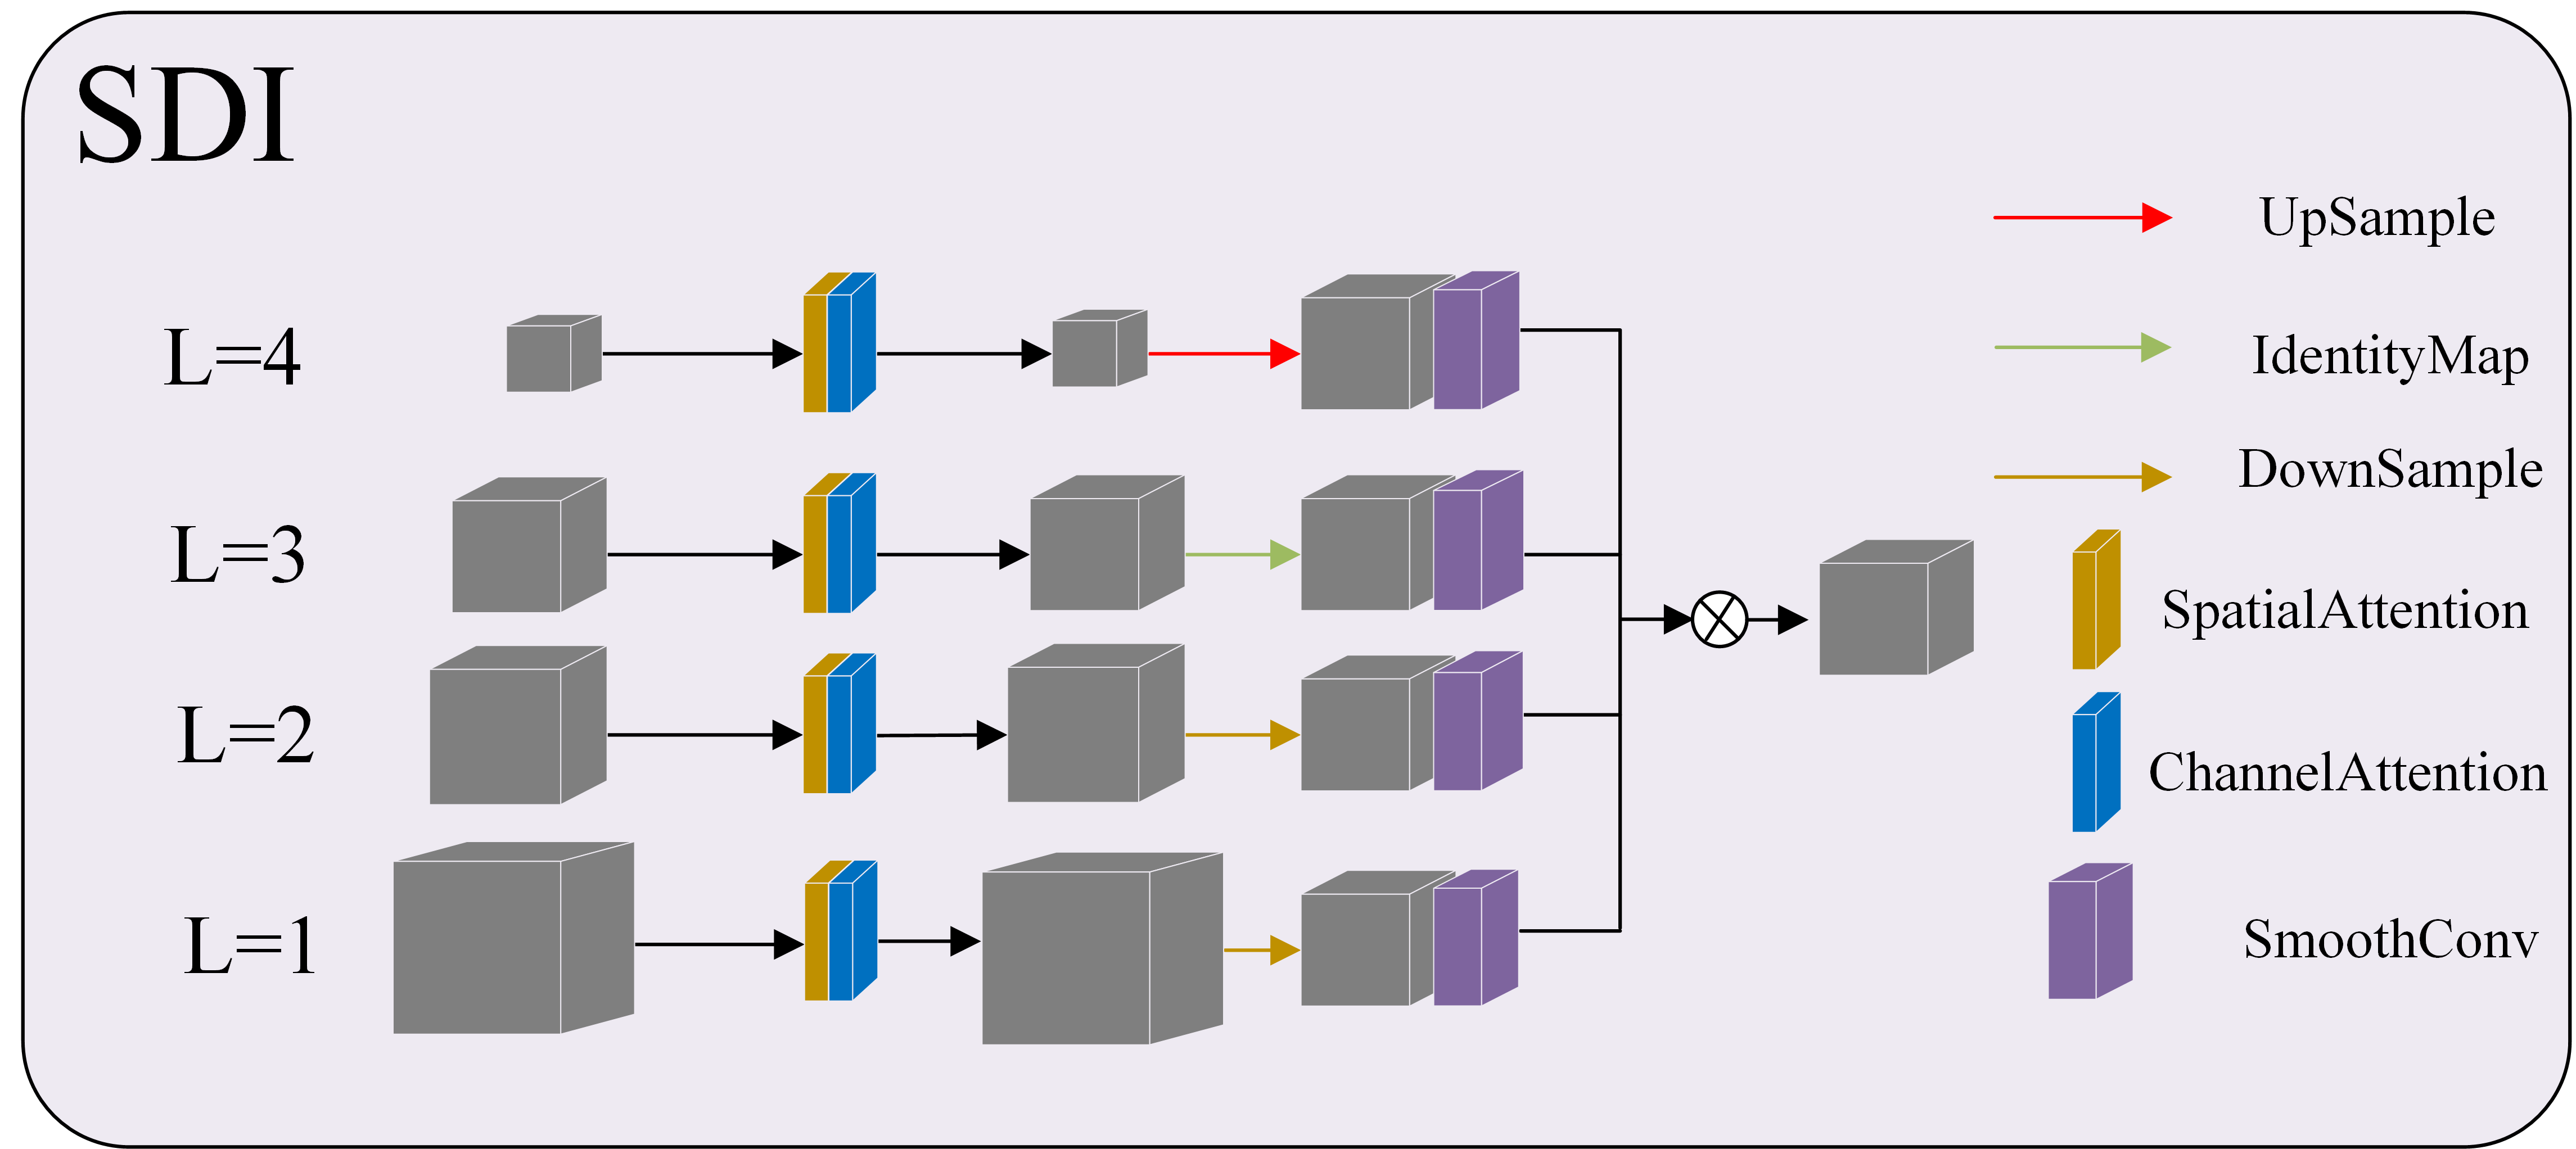
\includegraphics[width=0.8\textwidth]{images/sdi.png}
    \caption{Structure of the third layer skip connection module in CA-UNet} \label{sdi}
    \end{figure}

The SDI module first inputs the features $f_{i}^{0}$ of each level of the encoder into the CBAM module for spatial and channel attention, capturing and enhancing important feature information in the spatial and channel dimensions in depth, which is computed as follows:

\begin{equation}
	\begin{aligned}
		\label{eq:se1}
		f_{i}^{1}=\phi_{i}^{c}(\varphi_{i}^{s}(f_{i}^{0})), 
	\end{aligned}
\end{equation}where $f_{i}^{1}$ represents the feature map processed by the $ith$ level of the encoder, and $\phi_{i}^{c}$ and $\varphi_{i}^{s}$ respectively represent the parameters of the spatial and channel attention at the $ith$ level.


Afterwards, the $f_{i}^{1}$ layers with convolutional attention are aggregated and dimensionality reduced for channel information through a $1 \times 1$ convolution, resulting in the feature maps $f_{i}^{2} \in \mathbb{R}^{H_{i} \times W_{i} \times c}$ of each level.Next, the optimized features $f_{i}^{2}$ of each level are sent to the decoder. Specifically, at each decoder level $i$, $f_{i}^{2}$ is used as the target reference, and the size of each $jth$ level feature map is adjusted to match the same resolution of $f_{i}^{2}$, which is computed as follows:

\begin{equation}
	\begin{aligned}
		\label{eq:se2}
		f_{ij}^3=\begin{cases}\text{D}(f_j^2,(H_i,W_i))&\text{if} \quad j<i,\\\text{I}(f_j^2)&\text{if} \quad j=i,\\\text{U}(f_j^2,(H_i,W_i))&\text{if} \quad j>i,\end{cases}
	\end{aligned}
\end{equation}where $D(\cdot ),I(\cdot )$ and $U(\cdot )$ denote adaptive average pooling, identity mapping, and bilinear interpolation of $f_{j}^{2}$ to the resolution of $H_i \times W_i$.

Through a $3 \times 3$ convolution, each resampled feature map is smoothed into $f_{ij}^{3}$, which aims to reduce the potential jagged blurry features that may occur during the sampling process of the feature map. Lastly, a per-pixel Hadamard product is applied to all resampled and smoothed multi-level feature maps to enhance the feature maps of the $ith$ level in the decoder.


\section{Experiments}
\subsection{Datasets}
\textbf{Synapse dataset:}  The dataset includes 3779 axial abdominal clinical CT images from 30 cases. Each abdominal CT scan ranges from 85 to 198 CT slices of $512 \times 512$ pixels with voxel spatial resolution of $([0.54\sim 0.54] \times [0.98 \sim 0.98] \times [2.5 \sim 5.0])mm^3$. In this paper, following~\cite{chen2021transunet}, 18 CT case samples are divided into the training set, and the remaining 12 CT case samples are allocated to the test set. The average DSC and HD95 are used as the evaluation metrics to assess the segmentation performance of CA-UNet on 8 abdominal organs: Aorta, Gallbladder, Left Kidney, Right Kidney, Liver, Pancreas, Spleen, and Stomach.

%$\tnofoote{1 https://www.synapse.org/#!Synapse:syn3193805/wiki/217789}$
%$\footnote{2 https://www.creatis.insa-lyon.fr/Challenge/acdc/}$


\textbf{ACDC dataset:}  The dataset collects cardiac magnetic resonance imaging data from different patients using MRI scanners. The slice thickness of each MRI scan case is $5\sim8$ millimeters, covering the entire heart from the base to the top of the left ventricle. Additionally, the planar spatial resolution of these short-axis slices is between $0.83 \times 1.75 mm^2$/pixels. Each MRI scan case slice is professionally annotated in detail, including Left Ventricle (LV), Right Ventricle (LV), and myocardium (Myo). Following~\cite{chen2021transunet}, this dataset is randomly divided into 70 training samples (including 1930 axial slices), 10 validation samples, and 20 test samples. This paper uses average DSC to evaluate the performance of the algorithm proposed in this paper on the segmentation of 3 cardiac tissues.


\subsection{Implementation details}
The CA-UNet is implemented based on PyTorch and is trained and tested on the Nvidia GeForce RTX 4090 GPU. For each batch, the number of samples is set to 16 with a total of 400 iterations. Moreover, in this chapter, the number of channels $C$ of feature maps at all levels of the network model is set to 96, and the network model weights are randomly initialized and retrained. The AdamW optimizer is used, with the learning rate set to 0.001, momentum set to 0.9, and weight decay set to 1e-4. The data augmentation strategy follows MISSFormer~\cite{huang2022missformer}.


\begin{figure}[t!]
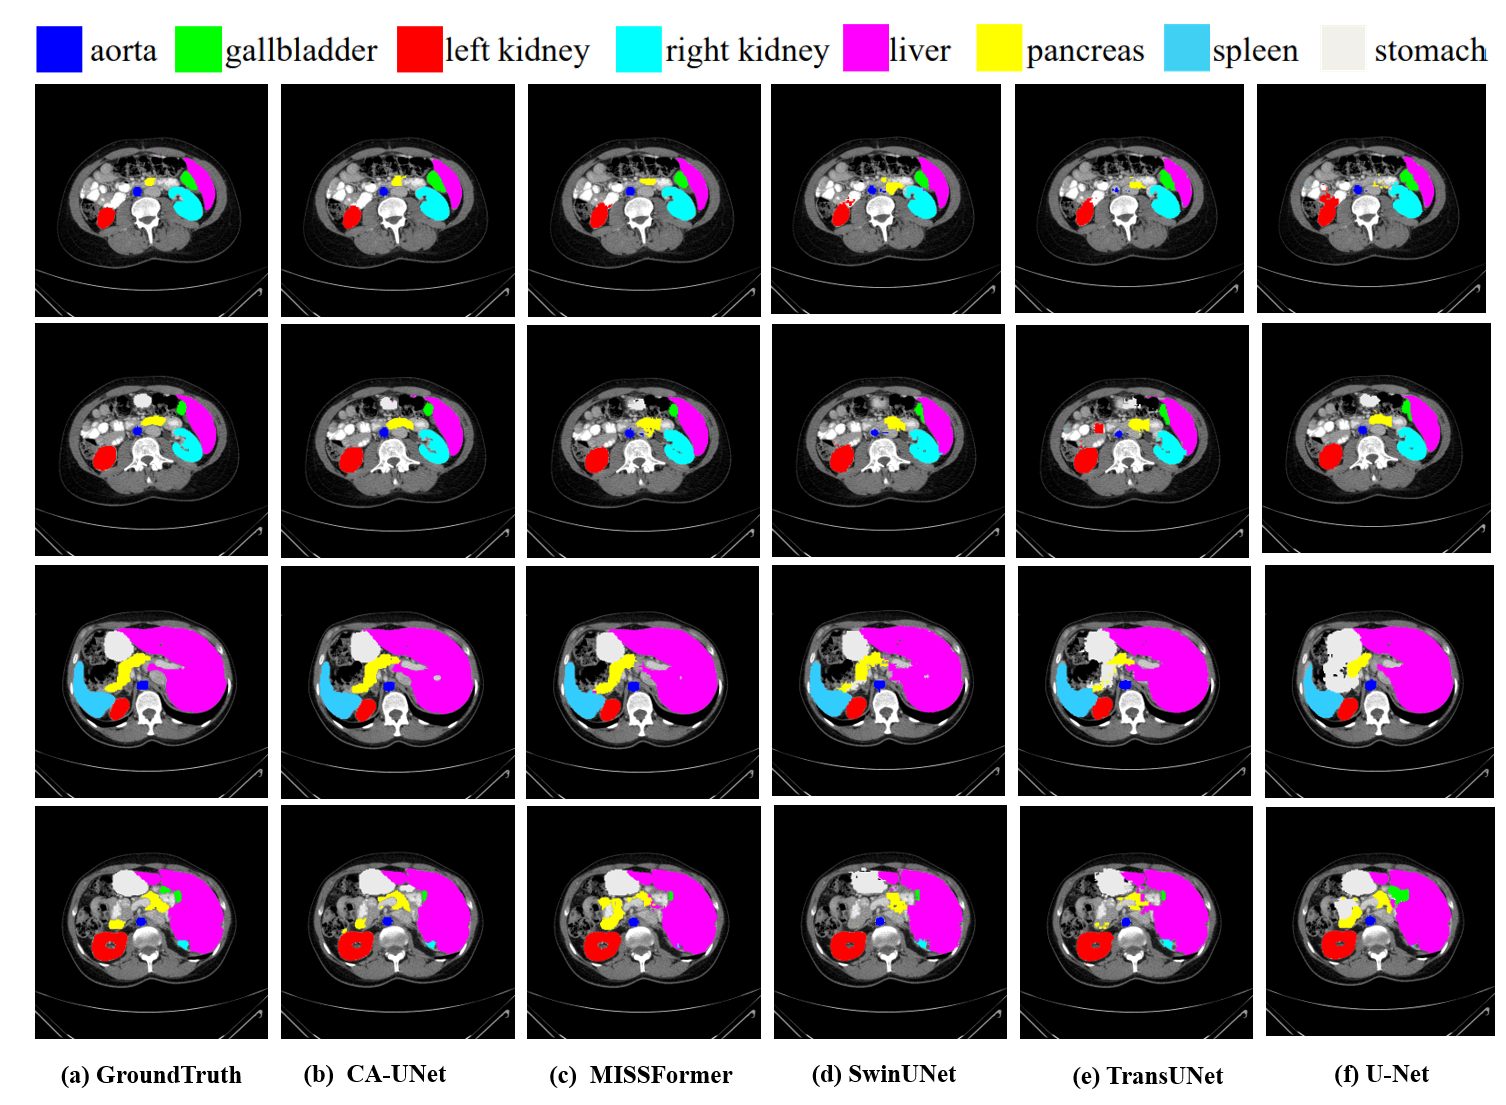
\includegraphics[width=\textwidth]{images/visulisation.png}
\caption{The segmentation visual results of different methods on the Synapse multi-organ CT dataset.}\label{segmentation}
\end{figure}



\subsection{Experiment results on Synapse dataset}

Table.~\ref{synapse} shows the quantitative comparison results of the segmentation accuracy (average DSC and HD95) of CA-UNet with the current mainstream methods.Experimental results demonstrate that our method achieves the best performance with segmentation accuracy of 84.43\%(DSC$\uparrow$) and 15.69($\downarrow$),respectively, showing an improvement of 1.88\% and 7.04\% compared to CASTformer~\cite{huang2022missformer}. Fig.~\ref{segmentation} shows a visual comparison of different methods on the Synapse multi-organ CT dataset. Compared to the current mainstream CNN-ViT or pure Transformer methods, our method demonstrates the excellence of the parallel heterogeneous feature extraction module. Even when substantially reducing the channel dimension of the feature map, it further optimizes the recognition accuracy of various organs and has higher clarity in edge segmentation.

\begin{table*}[htbp]
    \centering
    \caption{Segmentation accuracy of different methods on the Synapse dataset.}
    \footnotesize
    \resizebox{\textwidth}{!}{
    \begin{tabular}{c|cc|cccccccc}
    \hline
    Methods &  DSC$\uparrow$ &HD95$\downarrow$ & Aorta& Gallbladder& Kidney(L)& Kidney(R)& Liver& Pancreas& Spleen& Stomach\\
    \hline
    V-Net~\cite{milletari2016v} & 68.81 & - & 75.34 & 51.87 & 77.10 & 80.75 &
    87.84 & 40.05 & 80.56 & 56.98 \\
    DARR~\cite{fu2020domain} & 69.77 & - & 74.74 & 53.77 & 72.31 & 73.24 &
    94.08 & 54.18 & 89.90 & 45.96 \\
    R50 ViT~\cite{chen2021transunet} & 71.29 & 32.87 & 73.73 & 55.13 & 75.80 &
    72.20 & 91.51 & 45.99 & 81.99 & 73.95 \\
    R50 U-Net~\cite{chen2021transunet} & 74.68 & 36.87 & 84.18 & 62.84 & 79.19 &
    71.29 & 93.35 & 48.23 & 84.41 & 73.92 \\
    U-Net~\cite{ronneberger2015u} & 76.85 & 39.70 & 89.07 & 69.72 & 77.77 & 68.60 &
    93.43 & 53.98 & 86.67 & 75.58 \\
    TransUNet~\cite{chen2021transunet} & 77.48 & 31.69 & 87.23 & 63.13 & 81.87 &
    77.02 & 94.08 & 55.86 & 85.08 & 75.62 \\
    Att-UNet~\cite{oktay2018attention} & 77.77 & 36.02 & \textbf{89.55} & 68.88 & 77.98 &
    71.11 & 93.57 & 58.04 & 87.30 & 75.75 \\
    Swin UNet~\cite{cao2022swin} & 79.13 & 21.55 & 85.47 & 66.53 & 83.28 &
    79.61 & 94.29 & 56.58 & 90.66 & 76.60 \\
    MISSFormer~\cite{huang2022missformer} & 81.96 & 18.20 & 86.99 & 68.65 & 85.21 &
    82.00 & 94.41 & 65.67 & 91.92 & 80.81 \\
    CASTformer~\cite{you2022class} & 82.55 & 22.73 & 89.05 & 67.48 & 86.05 &
    82.17 & \textbf{95.61} & 67.49 & 91.00 & 81.55 \\
    \hline
    CA-UNet & \textbf{84.43} & \textbf{15.69} & 88.59 & \textbf{73.70} & \textbf{87.92} & \textbf{83.34} & 94.85 & 
    \textbf{71.52} & \textbf{91.98} & \textbf{82.51} \\
    \hline
    \end{tabular}
    }
    \label{synapse}
    \end{table*}


\subsection{Experiment results on ACDC dataset}

To validate the robustness and generalizability of CT-UNet on other medical datasets, we conducted training on the ACDC dataset in MRI mode, with experimental results shown in Table.~\ref{acdc}. The CA-UNet we proposed achieved 90.68\% accuracy in the segmentation of three types of cardiac tissues. The experimental results show that our method has reached an advanced level in the segmentation of Myo, while the segmentation performance for the LV and RV also reached a level comparable to the current mainstream method.
  
\begin{table}[htbp]
\caption{Segmentation accuracy of different methods on the ACDC dataset.}\label{acdc}
\begin{tabular}{c|c|ccc}
\hline
Methods & DSC& RV & Myo& LV\\
\hline
R50-U-Net~\cite{chen2021transunet} & 87.55 & 87.10 & 80.63 & 94.92\\
R50-AttnUNet~\cite{chen2021transunet} & 86.75 & 87.58 & 79.20 & 93.47\\
ViT-CUP~\cite{chen2021transunet} & 81.45 & 81.46 & 70.71 & 92.18\\
R50-ViT-CUP~\cite{chen2021transunet} & 87.57 & 86.07 & 81.88 & 94.75\\
TransUNet~\cite{chen2021transunet} & 89.71 & \textbf{88.86} & 84.53 & 95.73\\
Swin UNet~\cite{cao2022swin} & 90.00 & 88.55 & 85.62 & \textbf{95.83} \\
\hline
CA-UNet & \textbf{90.68} & 88.57 & \textbf{89.83} & 93.63 \\
\hline
\end{tabular}
\centering
\end{table}


\subsection{Ablation study}

Our proposed CA-UNet effectively aggregates a parallel heterogeneous module that fuses convolution and attention mechanisms, residual-structure-based downsampling, and full-scale skip connection based on CBAM. As a result, it demonstrates superior segmentation performance and generalization ability in medical imaging segmentation tasks. To verify its rationality and effectiveness, we conducted the following ablation experiment on the Synapse dataset.

\subsubsection{Effect of the parallel heterogeneous module:}

CA-UNet combines DwConv and self-attention in SwinTransformer to construct a parallel heterogeneous module for network hierarchical feature extraction and fusion, dynamically allocating weights adaptively in spatial position and channel dimensions. To verify its effectiveness, we examined whether the introduction of negligible computational cost deep convolution (for channel dimension feature capture) has an impact on segmentation performance. The ablation experiment results in Table.~\ref{phb} show that the average DSC of various organ segmentations was increased from 77.82\% to 84.43\%, a 3.97\% increase, through the designed hierarchical parallel heterogeneous module. This effectively enhances the recognition capability of complex medical image organs, making the edge segmentation more precise.

\begin{table}[htbp]
\caption{Ablation study on the effect of the parallel heterogeneous module:}\label{phb}
\footnotesize
\resizebox{\textwidth}{!}{
\begin{tabular}{c|c|cccccccc}
\hline
Methods &  DSC & Aorta& Gallbladder& Kidney(L)& Kidney(R)& Liver& Pancreas& Spleen& Stomach\\
\hline
$-$ DwConv & 80.38 & 87.54 & 68.35 & 78.77 & 77.48 & 93.99 & 66.53 & 89.43 & 80.93\\
$+$ DwConv & \textbf{84.43} & \textbf{88.59} & \textbf{73.70} & \textbf{87.92} & \textbf{83.34} & \textbf{94.85} & \textbf{71.52} & \textbf{91.98} & \textbf{82.51} \\
\hline
\end{tabular}
}
\centering
\end{table}

\subsubsection{Effect of downsampling module based on Res block:}

We incorporated the residual structure into the downsampling module, effectively enhancing the key detail features of the encoder feature maps at all scales and effectively avoiding the issue of feature location information loss caused by traditional downsampling methods (average pooling and max pooling). To validate its effectiveness, we explored the impact of using max pooling and Res block for downsampling on the segmentation performance of CA-UNet. The ablation experiment results in Table.~\ref{down} show that better segmentation precision was achieved through the downsampling module based on Res block, raising the average DSC from 79.55\% to 84.43\%.

\begin{table}[htbp]
\caption{Ablation study on the effect of downsampling module based on Res block}\label{down}
\footnotesize
\resizebox{\textwidth}{!}{
\begin{tabular}{c|c|cccccccc}
\hline
Downsampling &  DSC & Aorta& Gallbladder& Kidney(L)& Kidney(R)& Liver& Pancreas& Spleen& Stomach\\
\hline
Max pooling & 82.56 & 88.54 & 69.94 & 87.18 & 81.57 & 94.72 & 67.34 & 90.19 & 80.98\\
Residual structure & \textbf{84.43} & \textbf{88.59} & \textbf{73.70} & \textbf{87.92} & \textbf{83.34} & \textbf{94.85} & \textbf{71.52} & \textbf{91.98} & \textbf{82.51} \\
\hline
\end{tabular}
}
\centering
\end{table}

\subsubsection{Effect of the full-scale skip connection base on CBAM:}

We introduced a full-scale skip connection based on CBAM, which autonomously learns and aggregates the feature information of all levels of the encoder through spatial and channel attention, reducing the semantic gap caused by the blurring of feature mapping between the encoder and decoder. To explore its effectiveness, we discussed the impact of traditional skip connection based on channel dimension concatenation(CDC) and full-scale skip connection based on CBAM on network segmentation performance. The experimental results in Table.~\ref{skip} show that by introducing a full-scale skip connection based on CBAM, the segmentation accuracy of CA-UNet is effectively improved, raising the average DSC from 78.29\% to 84.43\%.

\begin{table}[htbp]
    \caption{Ablation study on the effect of downsampling module based on the residual structure}\label{skip}
    \footnotesize
    \resizebox{\textwidth}{!}{
    \begin{tabular}{c|c|cccccccc}
    \hline
    skip connection &  DSC & Aorta& Gallbladder& Kidney(L)& Kidney(R)& Liver& Pancreas& Spleen& Stomach\\
    \hline
    CDC & 80.09 & 87.11 & 70.45 & 79.35 & 74.11 & 94.34 & 63.53 & 90.16 & 81.69\\
    CBAM & \textbf{84.43} & \textbf{88.59} & \textbf{73.70} & \textbf{87.92} & \textbf{83.34} & \textbf{94.85} & \textbf{71.52} & \textbf{91.98} & \textbf{82.51} \\
    \hline
    \end{tabular}
    }
    \centering
    \end{table}

% \begin{table}[t!]
% \caption{Ablation study on the impact of the input size}\label{input}
% \footnotesize
% \resizebox{\textwidth}{!}{
% \begin{tabular}{c|c|cccccccc}
% \hline
% Input size &  DSC& Aorta& Gallbladder& Kidney(L)& Kidney(R)& Liver& Pancreas& Spleen& Stomach\\
% \hline
% 224 &  79.13& 85.47&66.53&83.28&79.61&94.29&56.58&\textbf{90.66}&\textbf{76.60}\\
% 384 &  \textbf{81.12} & \textbf{87.07}&\textbf{70.53}&\textbf{84.64}&\textbf{82.87}&\textbf{94.72}&\textbf{63.73}&90.14&75.29\\
% \hline
% \end{tabular}
% }
% \centering
% \end{table}

% \subsubsection{Effect of input size:}
% The testing results of the proposed Swin-Unet with $224\times224$, $384\times384$ input resolutions as input are presented in Table.~\ref{input}. As the input size increases from $224\times224$ to $384\times384$ and the patch size remains the same as $4$, the input token sequence of Transformer will become larger, thus leading to improve the segmentation performance of the model. However, although the segmentation accuracy of the model has been slightly improved, the computational load of the whole network has also increased significantly. In order to ensure the running efficiency of the algorithm, the experiments in this paper are based on $224\times224$ resolution scale as the input.


% \subsection{Discussion}

% As we all known, the performance of Transformer-based model is severely affected by model pre-training. In this work, we directly use the training weight of Swin transformer~\cite{swin} on ImageNet to initialize the network encoder and decoder, which may be a suboptimal scheme. This initialization approach is a simple one, and in the future we will explore the ways to pre-train Transformer end-to-end for medical image segmentation. Moreover, since the input images in this paper are 2D, while most of the medical image data are 3D, we will explore the application of Swin-Unet in 3D medical image segmentation in the following research.








\section{Conclusion}

In this paper, we effectively integrate CNN and Swin Transformer's window self-attention based on dynamic weight allocation mechanism, and designs CA block to enhance the sensitivity of the network to local features, as well as to extract and effectively fuse global feature information. Secondly, a downsampling module based on Res block and full-scale skip connection based on CBAM are designed to further enhance the model's ability to perceive complex details in medical images and understand abstract semantic information, thereby improving the clarity of edge segmentation. Finally, extensive experiments were conducted on two public medical image segmentation datasets. The experimental results validate that compared with previous state-of-the-art methods, CA-UNet has leading advantages in average DSC and HD95.




%
% ---- Bibliography ----
%
% BibTeX users should specify bibliography style 'splncs04'.
% References will then be sorted and formatted in the correct style.
%
% \bibliographystyle{splncs04}
% \bibliography{mybibliography}
%

\bibliographystyle{IEEEtran}
% argument is your BibTeX string definitions and bibliography database(s) 
\bibliography{CAUNet}


% \begin{thebibliography}{8}
% \bibitem{ref_article1}
% Author, F.: Article title. Journal \textbf{2}(5), 99--110 (2016)

% \bibitem{ref_lncs1}
% Author, F., Author, S.: Title of a proceedings paper. In: Editor,
% F., Editor, S. (eds.) CONFERENCE 2016, LNCS, vol. 9999, pp. 1--13.
% Springer, Heidelberg (2016). \doi{10.10007/1234567890}

% \bibitem{ref_book1}
% Author, F., Author, S., Author, T.: Book title. 2nd edn. Publisher,
% Location (1999)

% \bibitem{ref_proc1}
% Author, A.-B.: Contribution title. In: 9th International Proceedings
% on Proceedings, pp. 1--2. Publisher, Location (2010)

% \bibitem{ref_url1}
% LNCS Homepage, \url{http://www.springer.com/lncs}. Last accessed 4
% Oct 2017
% \end{thebibliography}

\end{document}
